%
% FH Technikum Wien
% !TEX encoding = UTF-8 Unicode
% LTeX: language=en
%
\documentclass[Proposal,english,IEEE]{twbook}
\usepackage[utf8]{inputenc}
\usepackage[T1]{fontenc}

% bitte setzen Sie hier den Studiengang
\degreecourse{MAI}

\addbibresource{Proposal.bib}

% Additional packages
\usepackage{blindtext}
\usepackage{pgfplots}
\usepackage{pgfplotstable}
\pgfplotsset{compat=1.18}
\usepackage{tikz}
\usetikzlibrary{shapes,arrows,positioning,calc}
\usepackage{booktabs}
\usepackage{multirow}
\usepackage{subcaption}
\usepackage{algorithm}
\usepackage{algpseudocode}
\usepackage{pgfplots}
\usepgfplotslibrary{fillbetween}

%
% Einträge für Deckblatt, Kurzfassung, etc.
%
\title{Playtesting Shattered Bonds Using Reinforcement Learning Agents For Automated Game Balancing}
\author{Nikolaus Rieder, B.Sc.}
\studentnumber{2410585040}
\supervisor{Julian Breddy}
\place{Vienna}

%---------------------------------------------------------------Abstract
\outline{%
This thesis investigates the application of deep reinforcement learning (DRL) agents for automated playtesting and game balancing in the action combat dungeon crawler \emph{Shattered Bonds}, developed in Unreal Engine 5. 
The research addresses the challenge of efficiently testing and balancing complex real-time combat mechanics—including movement, attack timing, ability usage, and defensive actions—without relying solely on expensive and time-consuming human playtesting. 
We propose a curriculum learning approach combined with carefully designed reward shaping to train agents capable of exhibiting human-like combat behaviors. 
The trained agents will generate telemetry data comparable to human playtesters, enabling rapid iteration on game balance parameters such as enemy difficulty, animation timing, and player survivability. 
MLOps practices will be explored for hyperparameter optimization of the reward function design. 
Expected outcomes include a reproducible framework for RL-based playtesting in Unreal Engine 5, quantitative metrics for difficulty assessment, and empirical comparison between agent and human playtesting data.
}

\keywords{Reinforcement Learning, Automated Playtesting, Game Balancing, Curriculum Learning, Reward Shaping, Unreal Engine 5, Deep Learning, Action Combat Games}

%---------------------------------------------------------------BEGIN
\begin{document}
%---------------------------------------------------------------TITLE
\maketitle

%---------------------------------------------------------------Motivation
\chapter{Motivation}

\section{Game Context: Shattered Bonds}

\emph{Shattered Bonds}\footnote{\url{https://store.steampowered.com/app/4191400/Shattered_Bonds/}} is an action combat dungeon crawler developed using Unreal Engine 5. The game features real-time combat mechanics that demand precise player inputs including:

\begin{itemize}
  \item \textbf{Movement and positioning}: Navigating 3D environments while avoiding hazards and enemy attacks
  \item \textbf{Attack timing}: Executing combo chains with precise timing windows
  \item \textbf{Ability usage}: Strategic deployment of special abilities with cooldowns
  \item \textbf{Defensive actions}: Blocking and parrying enemy attacks with frame-precise timing
\end{itemize}

The complexity of these interconnected systems creates a vast design space that is challenging to balance manually. Small changes to parameters such as enemy health, animation timing, damage values, or ability cooldowns can dramatically affect the player experience, potentially creating frustration points or trivializing content.

\section{The Game Balancing Challenge}

Game balancing in action combat games is notoriously difficult \cite{yannakakisRealTimeGameAdaptation2009}. Traditional approaches rely heavily on human playtesting, which suffers from several limitations:

\begin{enumerate}
  \item \textbf{Cost and scalability}: Human playtesters require compensation and cannot test continuously
  \item \textbf{Consistency}: Human performance varies based on fatigue, learning effects, and individual skill levels
  \item \textbf{Coverage}: Manual testing may miss edge cases or specific parameter combinations
  \item \textbf{Iteration speed}: Each balance change requires new playtesting sessions, slowing development
\end{enumerate}

The game industry has recognized automated playtesting as a potential solution \cite{gordilloImprovingPlaytestingCoverage2021, ferdousAgentBasedTesting3D2022}. Deep reinforcement learning (DRL) has shown promise in learning complex sequential decision-making tasks, including playing video games at superhuman levels \cite{ruppSimulationDrivenBalancingCompetitive2024}. However, applying DRL to action combat games for \emph{balancing} rather than merely \emph{winning} presents unique challenges.

\section{Relation to Master Thesis Topic}

This research sits at the intersection of several active areas in artificial intelligence and game development:

\begin{itemize}
  \item \textbf{Deep Reinforcement Learning}: Applying state-of-the-art algorithms (PPO, SAC) to complex continuous control tasks
  \item \textbf{Curriculum Learning}: Structuring training to progressively increase task difficulty \cite{CurriculumLearning2025}
  \item \textbf{Reward Engineering}: Designing reward functions that produce desired agent behaviors \cite{RewardShapingMastering}
  \item \textbf{Game AI and Testing}: Contributing to the growing field of AI-assisted game development \cite{lepelletierdewoillemontAutomatedPlayTestingRL2022}
  \item \textbf{MLOps for RL}: Exploring systematic approaches to hyperparameter optimization for reinforcement learning systems \cite{asc686f61MLFlowReinforcementLearning2025}
\end{itemize}

\section{Importance and Novelty}

While reinforcement learning has been applied to game testing \cite{ferdousAgentBasedTesting3D2022} and competitive game balancing \cite{ruppSimulationDrivenBalancingCompetitive2024}, several aspects make this research novel:

\begin{enumerate}
  \item \textbf{Real-time 3D combat}: Most RL playtesting research focuses on simpler 2D games or turn-based systems. Action combat in 3D presents significantly higher complexity in state and action spaces.

  \item \textbf{Multi-objective behavior}: The agent must learn not just to win, but to exhibit varied play styles that approximate human behavior for meaningful balance feedback.

  \item \textbf{Unreal Engine 5 integration}: Establishing a reproducible framework for RL training within UE5, building on recent developments like Learning Agents \cite{AlanLaboratoryUnrealMLAgents2025}.

  \item \textbf{Production game context}: Unlike most academic work using simplified environments, this research operates on an actual commercial game in active development.

  \item \textbf{Comparative telemetry}: Direct comparison of agent-generated and human playtester data using identical data collection infrastructure.
\end{enumerate}

\section{Research Question}

Based on the challenges and opportunities outlined above, this thesis addresses the following research question:

\begin{quote}
  \textbf{RQ:} \emph{How can curriculum learning and reward shaping be combined to train deep reinforcement learning agents that generate playtesting data comparable to human testers for balancing real-time combat mechanics in a 3D action game, and what metrics effectively quantify the resulting balance quality?}
\end{quote}

This question encompasses several sub-questions:
\begin{itemize}
  \item What curriculum structure enables efficient learning of complex combat behaviors?
  \item How should rewards be designed to encourage diverse, human-like play styles rather than purely optimal play?
  \item What telemetry metrics best capture difficulty and balance characteristics?
  \item How do agent-generated metrics compare to human playtester data statistically?
\end{itemize}

%---------------------------------------------------------------Literature Review
\chapter{Literature Review}

\section{Reinforcement Learning for Game Testing}

The application of reinforcement learning to game testing has gained significant attention in recent years. Bergdahl et al. demonstrated that deep reinforcement learning can augment automated game testing by learning to explore game mechanics and detect bugs without explicit scripting \cite{gordilloImprovingPlaytestingCoverage2021}. Their work on curiosity-driven exploration showed that RL agents can achieve meaningful test coverage in complex 3D environments.

Ferdous et al. \cite{ferdousAgentBasedTesting3D2022} presented an approach for agent-based testing of 3D games using curiosity as a motivating factor. Their results provide preliminary evidence that RL can be adopted for automated testing, though they note challenges with complex game mechanics.

The Wuji framework represents a significant advancement, combining evolutionary algorithms with deep reinforcement learning for combat game testing. Zheng et al. demonstrated that this hybrid approach could discover bugs in commercial games by balancing between task completion and state space exploration. Their multi-objective optimization approach is particularly relevant to our work.

\section{Game Balancing with Machine Learning}

Rupp et al. \cite{ruppSimulationDrivenBalancingCompetitive2024} proposed simulation-driven balancing using reinforcement learning within the PCGRL framework. Their architecture separates level generation from balancing, with a reward model based on simulation outcomes. While focused on tile-based competitive games, their methodology of using repeated simulations to assess balance informs our approach.

Noblega et al. \cite{noblegaAdaptiveDeepReinforcement2025} explored adaptive deep reinforcement game balancing, proposing reward functions based on balancing constants. Their work demonstrates that RL agents can maintain balance while adapting to different player skill levels.

Yannakakis and Hallam \cite{yannakakisRealTimeGameAdaptation2009} established foundational work on real-time game adaptation for player satisfaction, using neural networks to model player preferences and adapt game parameters accordingly.

\section{Automated Play-Testing with Human-Like Behavior}

Le Pelletier De Woillemont et al. \cite{lepelletierdewoillemontAutomatedPlayTestingRL2022} introduced CARMI (Configurable Agent with Relative Metrics as Input), an agent capable of emulating human play styles for automated testing. Unlike methods requiring full gameplay trajectories, CARMI uses summary data, making it practical for production environments. This approach to generating human-like behaviors is central to our methodology.

\section{Curriculum Learning in Reinforcement Learning}

Curriculum learning \cite{CurriculumLearning2025} structures training by progressively increasing task difficulty. In RL contexts, this has proven effective for complex tasks where naive training fails to converge. OpenAI's work on Dota 2 and DeepMind's AlphaStar both employed curriculum strategies to achieve superhuman performance in complex games.

For game testing specifically, curriculum learning offers a path to training agents that can handle the full complexity of combat systems by first mastering simpler sub-tasks.

\section{Multi-Agent Reinforcement Learning}

Buşoniu et al. \cite{busoniuMultiagentReinforcementLearning2010} provide a comprehensive overview of multi-agent RL, discussing cooperative, competitive, and mixed scenarios. Tan's foundational work \cite{tanMultiAgentReinforcementLearning1993} on independent versus cooperative agents established key principles for multi-agent systems.

Papoudakis et al. \cite{papoudakisDealingNonStationarityMultiAgent2019} address the non-stationarity problem in multi-agent deep RL, surveying methods from centralized training to meta-learning. These insights are relevant if we pursue a multi-agent architecture where different agents specialize in different combat aspects.

\section{Research Gap}

Despite significant progress, several gaps remain that this thesis addresses:

\begin{enumerate}
  \item \textbf{Real-time 3D action combat}: Most work focuses on turn-based, 2D, or strategy games rather than real-time 3D combat with precise timing requirements.

  \item \textbf{Balance-focused rather than win-focused}: Existing RL game agents optimize for winning; our work requires agents that produce useful balance feedback.

  \item \textbf{Unreal Engine 5 integration}: Limited academic work exists on RL integration with UE5 for production games.

  \item \textbf{Comparative validation}: Few studies compare RL-generated telemetry directly with human playtester data using statistical methods.
\end{enumerate}

%---------------------------------------------------------------Proposed Methods
\chapter{Proposed Methods}

\section{Overview}

The proposed methodology consists of four main components:

\begin{enumerate}
  \item \textbf{Environment Design}: Creating training environments within Unreal Engine 5
  \item \textbf{Agent Architecture}: Designing the RL agent(s) for combat control
  \item \textbf{Training Pipeline}: Implementing curriculum learning and reward shaping
  \item \textbf{Evaluation Framework}: Collecting and analyzing telemetry data
\end{enumerate}

\section{Data Sources}

\subsection{Training Data}

The agent learns through interaction with the game environment. No pre-recorded human gameplay is required for training, though human data serves as validation:

\begin{itemize}
  \item \textbf{State observations}: Player position, health, stamina, enemy positions and states, ability cooldowns, animation states
  \item \textbf{Actions}: Movement direction/magnitude, attack commands, ability activation, block/parry inputs
  \item \textbf{Rewards}: Designed reward signals (see Section~\ref{sec:reward})
\end{itemize}

\subsection{Validation Data}

For comparison with human behavior:

\begin{itemize}
  \item \textbf{Firestore telemetry}: The game's existing backend collects gameplay events from all sessions
  \item \textbf{Human playtester sessions}: Controlled playtesting sessions with standardized scenarios
  \item \textbf{Agent sessions}: Identical scenarios played by trained agents
\end{itemize}

Telemetry events include:
\begin{itemize}
  \item Encounter completion time
  \item Number of deaths/retries
  \item Health lost per encounter
  \item Ability usage frequency and timing
  \item Damage dealt vs. damage taken ratios
  \item Block/parry success rates
\end{itemize}

\section{Methods}

\subsection{Environment Design}

Custom training environments will be created in Unreal Engine 5:

\begin{enumerate}
  \item \textbf{Isolated combat arenas}: Controlled spaces for curriculum stages
  \item \textbf{Standardized enemy encounters}: Reproducible combat scenarios
  \item \textbf{Parameterized difficulty}: Adjustable enemy stats, timing windows, and spawn configurations
\end{enumerate}

Integration options under consideration:
\begin{itemize}
  \item \textbf{UE5 Learning Agents}: Epic's official ML plugin for reinforcement and imitation learning
  \item \textbf{Unreal ML-Agents}: Community port of Unity ML-Agents \cite{AlanLaboratoryUnrealMLAgents2025}
  \item \textbf{Custom Python bridge}: Direct socket communication for maximum flexibility
\end{itemize}

\subsection{Agent Architecture}

The primary approach uses a single agent controlling all combat aspects. A secondary experimental approach may explore multi-agent decomposition:

\textbf{Single Agent (Primary):}
\begin{itemize}
  \item Policy network: Actor-critic architecture with shared feature extraction
  \item Algorithm: Proximal Policy Optimization (PPO) or Soft Actor-Critic (SAC)
  \item Observation space: Vector encoding of game state (position, health, enemies, cooldowns)
  \item Action space: Continuous (movement) + discrete (combat actions) hybrid
\end{itemize}

\textbf{Multi-Agent (Experimental):}
\begin{itemize}
  \item Movement agent: Handles positioning and navigation
  \item Combat agent: Controls attack timing and combos
  \item Ability agent: Manages special ability usage
  \item Defense agent: Handles blocking and parrying
  \item Coordinator: Arbitrates between agent outputs
\end{itemize}

\subsection{Curriculum Learning}

Training progresses through stages of increasing complexity:

\begin{enumerate}
  \item \textbf{Stage 1 — Movement}: Navigate to targets, avoid static hazards
  \item \textbf{Stage 2 — Basic Combat}: Attack stationary training dummies
  \item \textbf{Stage 3 — Timing}: Hit moving targets with timing windows
  \item \textbf{Stage 4 — Defense}: Block/parry predictable attacks
  \item \textbf{Stage 5 — Single Enemy}: Full combat against one enemy type
  \item \textbf{Stage 6 — Multiple Enemies}: Handle multiple simultaneous threats
  \item \textbf{Stage 7 — Full Encounters}: Complete dungeon encounters
\end{enumerate}

Progression criteria based on success rate thresholds (e.g., 80\% success before advancing).

\subsection{Reward Shaping}
\label{sec:reward}

Reward design balances multiple objectives:

\begin{equation}
  R_{total} = w_1 R_{survival} + w_2 R_{damage} + w_3 R_{efficiency} + w_4 R_{exploration} + R_{sparse}
\end{equation}

Where:
\begin{itemize}
  \item $R_{survival}$: Positive reward for maintaining health, penalty for damage taken
  \item $R_{damage}$: Reward for dealing damage to enemies
  \item $R_{efficiency}$: Reward for completing objectives quickly
  \item $R_{exploration}$: Intrinsic curiosity reward for state coverage
  \item $R_{sparse}$: Large rewards for encounter completion, penalties for death
\end{itemize}

Weight optimization will explore:
\begin{itemize}
  \item Manual tuning with ablation studies
  \item Learned reward shaping using a secondary network
  \item Hyperparameter optimization (grid search, Bayesian optimization)
\end{itemize}

\subsection{MLOps Integration}

Experiment tracking and hyperparameter optimization:

\begin{itemize}
  \item \textbf{MLflow} \cite{asc686f61MLFlowReinforcementLearning2025}: Track training runs, log metrics, version models
  \item \textbf{Weights \& Biases}: Visualize training progress, compare experiments
  \item \textbf{Optuna}: Automated hyperparameter search for reward weights and network architecture
\end{itemize}

\section{Milestones}

\begin{table}[htbp]
  \centering
  \caption{Project Milestones and Timeline}
  \label{tab:milestones}
  \begin{tabular}{@{}clp{6cm}c@{}}
    \toprule
    \textbf{MS} & \textbf{Phase} & \textbf{Deliverable}                                                       & \textbf{Target} \\
    \midrule
    1           & Setup          & UE5-Python communication established, basic agent training loop functional & Month 1         \\
    \addlinespace
    2           & Environment    & Training arenas created, telemetry pipeline integrated with Firestore      & Month 1         \\
    \addlinespace
    3           & Curriculum     & Stages 1--4 implemented, agent learns basic movement and combat            & Month 2         \\
    \addlinespace
    4           & Full Training  & All curriculum stages complete, agent completes full encounters            & Month 2         \\
    \addlinespace
    5           & Human Data     & Controlled playtesting sessions conducted, human baseline established      & Month 3         \\
    \addlinespace
    6           & Analysis       & Statistical comparison complete, metrics validated                         & Month 3         \\
    \addlinespace
    7           & Optimization   & Reward shaping optimized, MLOps pipeline functional                        & Month 4         \\
    \addlinespace
    8           & Thesis         & Written thesis submitted                                                   & Month 4         \\
    \bottomrule
  \end{tabular}
\end{table}

%---------------------------------------------------------------Expected Results
\chapter{Expected Results}

\section{Evaluation Metrics}

\subsection{Training Metrics}

Metrics to assess agent learning progress:

\begin{itemize}
  \item \textbf{Episode reward}: Cumulative reward per episode over training
  \item \textbf{Success rate}: Percentage of encounters completed successfully
  \item \textbf{Curriculum progression}: Time/episodes to advance through stages
  \item \textbf{Policy entropy}: Measure of action diversity (higher = more exploration)
\end{itemize}

\subsection{Gameplay Metrics}

Metrics capturing combat performance and difficulty:

\begin{itemize}
  \item \textbf{Encounter completion time}: Time to defeat all enemies
  \item \textbf{Death count}: Number of player deaths per encounter
  \item \textbf{Health efficiency}: $\frac{\text{Final Health}}{\text{Starting Health}}$
  \item \textbf{Damage ratio}: $\frac{\text{Damage Dealt}}{\text{Damage Taken}}$
  \item \textbf{Ability utilization}: Frequency and timing of ability usage
  \item \textbf{Defensive success rate}: $\frac{\text{Successful Blocks/Parries}}{\text{Total Defensive Attempts}}$
  \item \textbf{Hit rate}: $\frac{\text{Attacks Landed}}{\text{Attacks Attempted}}$
\end{itemize}

\subsection{Balance Metrics}

Metrics specifically for assessing game balance:

\begin{itemize}
  \item \textbf{Difficulty index}: Composite score combining death rate, completion time, and health loss
  \item \textbf{Frustration indicator}: Repeated deaths in same location/encounter
  \item \textbf{Trivial encounter detection}: Encounters completed with minimal health loss
  \item \textbf{Balance variance}: Consistency of difficulty across similar encounters
\end{itemize}

\section{Visualization: Plot Types}

\subsection{Training Progress}

\begin{figure}[htbp]
  \centering
  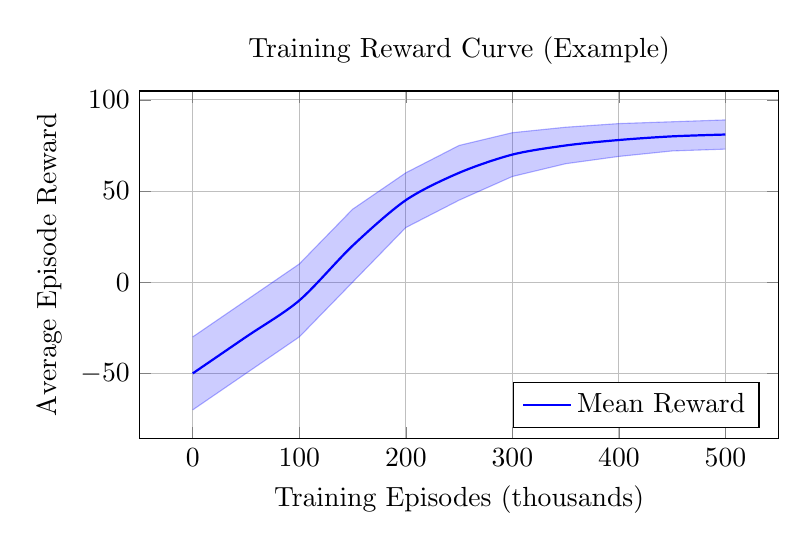
\begin{tikzpicture}
    \begin{axis}[
        width=0.8\textwidth,
        height=6cm,
        xlabel={Training Episodes (thousands)},
        ylabel={Average Episode Reward},
        title={Training Reward Curve (Example)},
        grid=major,
        legend pos=south east,
      ]
      % Dummy data showing typical RL training curve
      \addplot[blue, thick, smooth] coordinates {
          (0, -50) (50, -30) (100, -10) (150, 20) (200, 45)
          (250, 60) (300, 70) (350, 75) (400, 78) (450, 80) (500, 81)
        };
      \addlegendentry{Mean Reward}

      \addplot[blue, opacity=0.3, name path=upper] coordinates {
          (0, -30) (50, -10) (100, 10) (150, 40) (200, 60)
          (250, 75) (300, 82) (350, 85) (400, 87) (450, 88) (500, 89)
        };
      \addplot[blue, opacity=0.3, name path=lower] coordinates {
          (0, -70) (50, -50) (100, -30) (150, 0) (200, 30)
          (250, 45) (300, 58) (350, 65) (400, 69) (450, 72) (500, 73)
        };
      \addplot[blue, opacity=0.2] fill between[of=upper and lower];
    \end{axis}
  \end{tikzpicture}
  \caption{Example training reward curve with confidence interval}
  \label{fig:training_reward}
\end{figure}

\subsection{Human vs. Agent Comparison}

\begin{figure}[htbp]
  \centering
  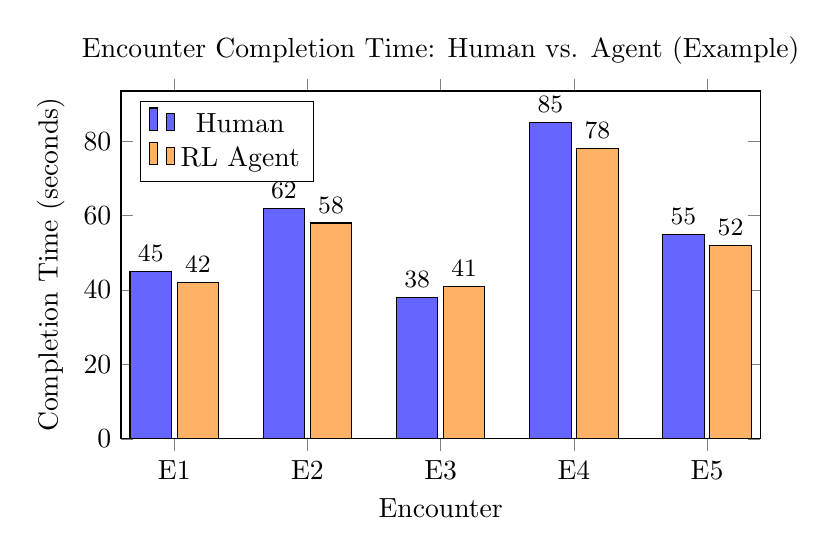
\begin{tikzpicture}
    \begin{axis}[
        width=0.8\textwidth,
        height=6cm,
        ybar,
        bar width=15pt,
        xlabel={Encounter},
        ylabel={Completion Time (seconds)},
        title={Encounter Completion Time: Human vs. Agent (Example)},
        symbolic x coords={E1, E2, E3, E4, E5},
        xtick=data,
        legend pos=north west,
        ymin=0,
        nodes near coords,
        every node near coord/.append style={font=\small},
      ]
      \addplot[fill=blue!60] coordinates {(E1, 45) (E2, 62) (E3, 38) (E4, 85) (E5, 55)};
      \addplot[fill=orange!60] coordinates {(E1, 42) (E2, 58) (E3, 41) (E4, 78) (E5, 52)};
      \legend{Human, RL Agent}
    \end{axis}
  \end{tikzpicture}
  \caption{Example comparison of completion times across encounters}
  \label{fig:completion_comparison}
\end{figure}

\subsection{Difficulty Spike Detection}

\begin{figure}[htbp]
  \centering
  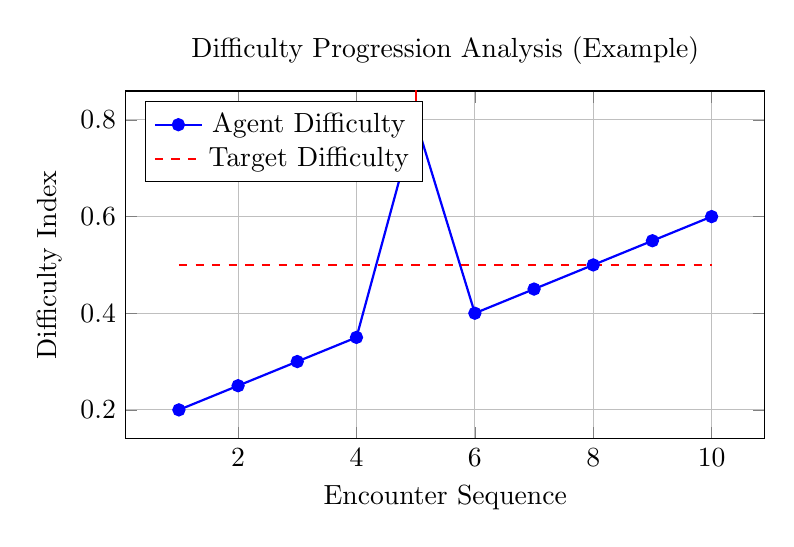
\begin{tikzpicture}
    \begin{axis}[
        width=0.8\textwidth,
        height=6cm,
        xlabel={Encounter Sequence},
        ylabel={Difficulty Index},
        title={Difficulty Progression Analysis (Example)},
        grid=major,
        legend pos=north west,
      ]
      \addplot[blue, thick, mark=*] coordinates {
          (1, 0.2) (2, 0.25) (3, 0.3) (4, 0.35) (5, 0.8)
          (6, 0.4) (7, 0.45) (8, 0.5) (9, 0.55) (10, 0.6)
        };
      \addlegendentry{Agent Difficulty}

      \addplot[red, dashed, thick] coordinates {(1, 0.5) (10, 0.5)};
      \addlegendentry{Target Difficulty}

      \node[pin={[pin edge={red,thick}]90:{\textbf{Difficulty Spike!}}}] at (axis cs:5,0.8) {};
    \end{axis}
  \end{tikzpicture}
  \caption{Example difficulty progression showing detected spike at Encounter 5}
  \label{fig:difficulty_spike}
\end{figure}

\subsection{Metric Distribution Comparison}

\begin{figure}[htbp]
  \centering
  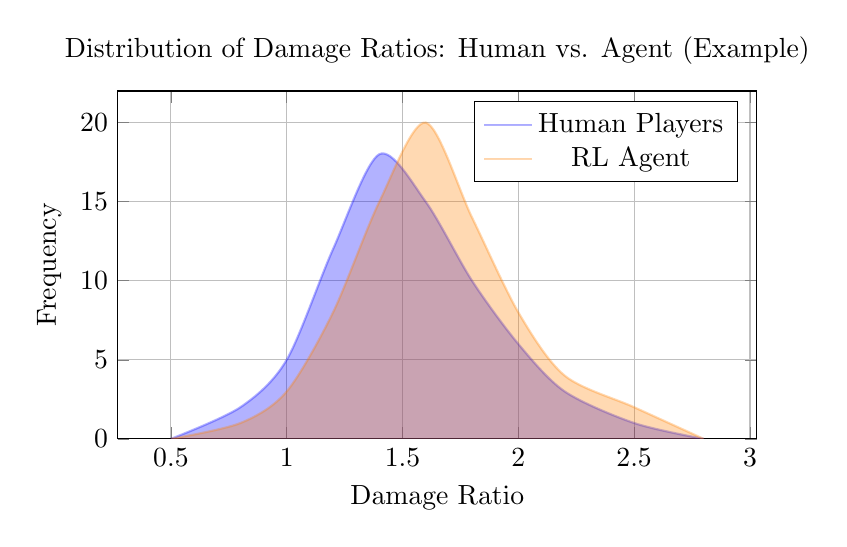
\begin{tikzpicture}
    \begin{axis}[
        width=0.8\textwidth,
        height=6cm,
        xlabel={Damage Ratio},
        ylabel={Frequency},
        title={Distribution of Damage Ratios: Human vs. Agent (Example)},
        grid=major,
        legend pos=north east,
        ymin=0,
      ]
      % Human distribution (dummy normal-ish)
      \addplot[blue, thick, smooth, fill=blue, opacity=0.3] coordinates {
          (0.5, 0) (0.8, 2) (1.0, 5) (1.2, 12) (1.4, 18)
          (1.6, 15) (1.8, 10) (2.0, 6) (2.2, 3) (2.5, 1) (2.8, 0)
        };
      \addlegendentry{Human Players}

      % Agent distribution (dummy, slightly different)
      \addplot[orange, thick, smooth, fill=orange, opacity=0.3] coordinates {
          (0.5, 0) (0.8, 1) (1.0, 3) (1.2, 8) (1.4, 15)
          (1.6, 20) (1.8, 14) (2.0, 8) (2.2, 4) (2.5, 2) (2.8, 0)
        };
      \addlegendentry{RL Agent}
    \end{axis}
  \end{tikzpicture}
  \caption{Example distribution comparison for statistical testing}
  \label{fig:distribution}
\end{figure}

\section{Statistical Tests}

To validate that agent behavior approximates human behavior and to assess statistical significance of balance findings:

\subsection{Comparing Distributions}

\begin{itemize}
  \item \textbf{Kolmogorov-Smirnov test}: Compare cumulative distributions of metrics between human and agent populations
  \item \textbf{Mann-Whitney U test}: Non-parametric comparison of medians when distributions are non-normal
  \item \textbf{Welch's t-test}: Compare means when normality assumption holds
\end{itemize}

\subsection{Correlation Analysis}

\begin{itemize}
  \item \textbf{Pearson correlation}: Linear relationship between agent and human metrics
  \item \textbf{Spearman correlation}: Rank-order correlation for non-linear relationships
\end{itemize}

\subsection{Effect Size}

\begin{itemize}
  \item \textbf{Cohen's d}: Quantify magnitude of differences between groups
  \item \textbf{95\% Confidence intervals}: Uncertainty bounds on all reported metrics
\end{itemize}

\subsection{Balance-Specific Tests}

\begin{itemize}
  \item \textbf{ANOVA}: Compare difficulty across multiple encounter types
  \item \textbf{Chi-square test}: Analyze categorical outcomes (success/failure patterns)
  \item \textbf{Regression analysis}: Model difficulty as function of game parameters
\end{itemize}

\section{Expected Outcomes}

\subsection{Primary Deliverables}

\begin{enumerate}
  \item \textbf{Trained RL Agent}: An agent capable of completing combat encounters in \emph{Shattered Bonds} with measurable success rates

  \item \textbf{UE5 Training Framework}: Documented codebase for RL training in Unreal Engine 5, potentially reusable for similar projects

  \item \textbf{Telemetry Analysis Pipeline}: Tools for comparing agent and human gameplay data

  \item \textbf{Balance Recommendations}: Data-driven insights on encounter difficulty and potential balance issues
\end{enumerate}

\subsection{Research Contributions}

\begin{enumerate}
  \item Empirical evaluation of curriculum learning effectiveness for complex 3D combat

  \item Methodology for reward shaping that produces human-comparable behaviors

  \item Statistical framework for validating RL playtesting against human baselines

  \item Practical guidelines for integrating RL playtesting into game production
\end{enumerate}

\subsection{Limitations and Risks}

\begin{itemize}
  \item \textbf{Training time}: Complex environments may require substantial compute resources
  \item \textbf{Sim-to-real gap}: Agent behavior in training may not transfer perfectly to all game scenarios
  \item \textbf{Human data quantity}: Limited human playtester availability may constrain statistical power
  \item \textbf{UE5 integration complexity}: Technical challenges with engine integration may require fallback approaches
\end{itemize}

%---------------------------------------------------------------Bibliography
\clearpage
\printbibliography
\clearpage

% Das Abbildungsverzeichnis
\listoffigures
\clearpage

% Das Tabellenverzeichnis
\listoftables
\clearpage

% Das Verzeichnis über die verwendeten KI-Tools
\listaitools
\clearpage

\phantomsection
\addcontentsline{toc}{chapter}{\listacroname}
\chapter*{\listacroname}
\begin{acronym}[XXXXX]
  \acro{RL}[RL]{Reinforcement Learning}
  \acro{DRL}[DRL]{Deep Reinforcement Learning}
  \acro{PPO}[PPO]{Proximal Policy Optimization}
  \acro{SAC}[SAC]{Soft Actor-Critic}
  \acro{UE5}[UE5]{Unreal Engine 5}
  \acro{DDA}[DDA]{Dynamic Difficulty Adjustment}
  \acro{MARL}[MARL]{Multi-Agent Reinforcement Learning}
  \acro{MLOps}[MLOps]{Machine Learning Operations}
  \acro{NPC}[NPC]{Non-Player Character}
  \acro{API}[API]{Application Programming Interface}
\end{acronym}

\end{document}